\subsection*{Problema 45}

\textbf{Enunciado:}
Calcular la integral indefinida:
\begin{align*}
\int \dfrac{x}{\sqrt{x - 1}} \, dx
\end{align*}

\textbf{Solución:}
Para resolver la integral, aplicamos el método de sustitución recomendado. Definimos la nueva variable $u$:
\begin{align*}
u &= \sqrt{x - 1}
\end{align*}

Elevamos al cuadrado ambos lados para despejar la variable $x$:
\begin{align*}
u^2 &= x - 1 \\
x &= u^2 + 1
\end{align*}

Ahora, encontramos el diferencial $dx$ derivando la expresión de $x$ con respecto a $u$:
\begin{align*}
dx &= 2u \, du
\end{align*}

Sustituimos $x$, $\sqrt{x-1}$ y $dx$ en la integral original:
\begin{align*}
\int \dfrac{u^2 + 1}{u} (2u \, du)
\end{align*}

Simplificamos la expresión algebraica cancelando $u$ y extrayendo las constantes:
\begin{align*}
&= \int (u^2 + 1)(2) \, du \\
&= 2 \int (u^2 + 1) \, du
\end{align*}

integramos término a término usando la regla de la potencia:
\begin{align*}
&= 2 \left( \dfrac{u^3}{3} + u \right) + C
\end{align*}

Distribuimos el factor 2:
\begin{align*}
&= \dfrac{2}{3}u^3 + 2u + C
\end{align*}

Finalmente, regresamos a la variable original $x$ sustituyendo $u = \sqrt{x - 1}$:
\begin{align*}
&= \dfrac{2}{3}(\sqrt{x - 1})^3 \\
&\quad + 2\sqrt{x - 1} + C
\end{align*}

Agrupando el resultado, la solución general es:
\begin{align*}
\int \dfrac{x}{\sqrt{x - 1}} \, dx = \dfrac{2}{3}(x - 1)^{\frac{3}{2}} \\
+ 2(x - 1)^{\frac{1}{2}} + C
\end{align*}

\begin{figure}[H]
	\centering
	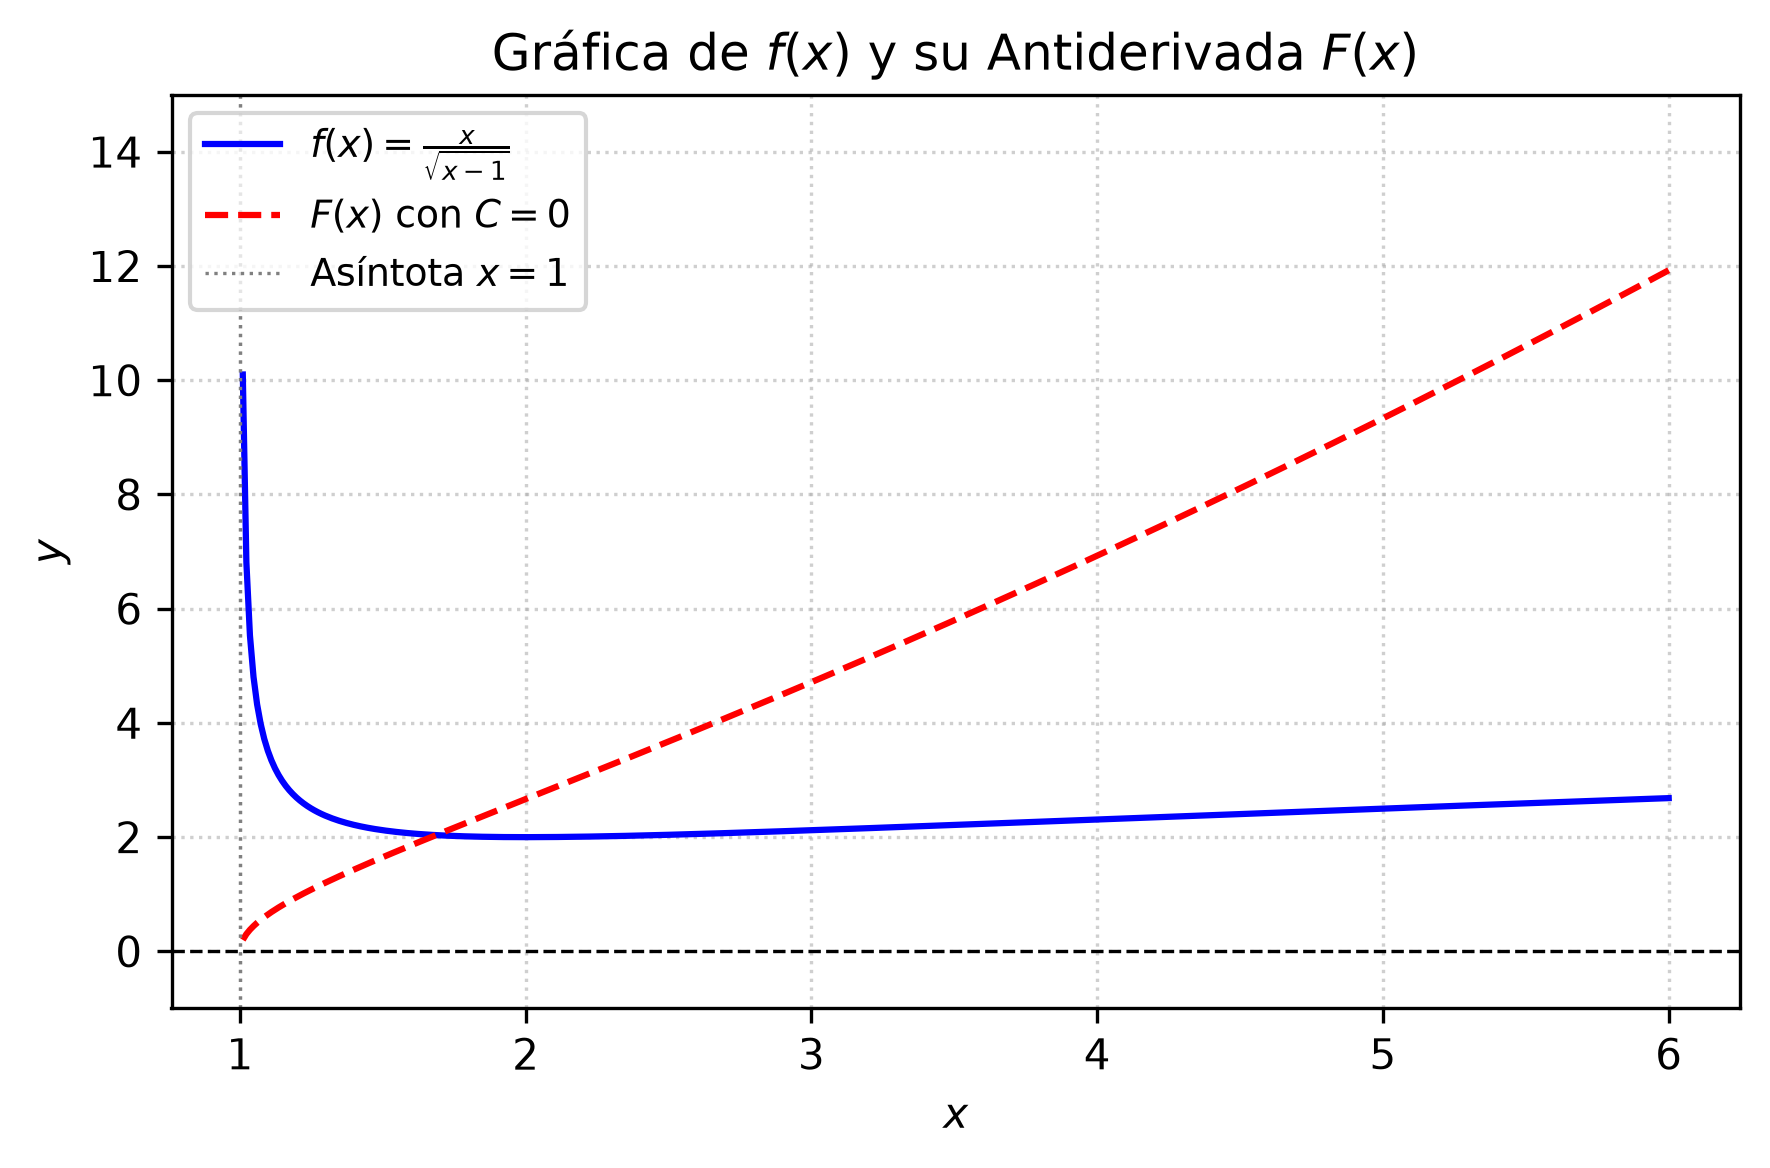
\includegraphics[width=\columnwidth]{semana_05/graficas/SEM05_P45_grafica.png}
	\caption{Representación gráfica de $f(x)$ y su antiderivada $F(x)$ evaluada para la constante de integración $C = 0$ (Problema 45).}
	\label{fig:problema45}
\end{figure}
